% !TeX root = 00_Vorlage.tex
% !TeX spellcheck = de_DE
\chapter{Ergebnisse}
\label{sec:ergebnisse}

Im folgenden Abschnitt werden die Ergebnisse der Massenbestimmungen und der anschließenden Versuchen mit einer und mehrerer Federn. Alle Fehlerangaben beziehen sich auf statistische Fehler; Systematische werden gegebenenfalls separat diskutiert. 

\section{Massenbestimmung}
Die Masse des Pendelkörpers wurde über eine simultane Kraft- und Beschleunigungsmessung und Newtons Axiom \autoref{eqn:newt} bestimmt. In \autoref{fig:mass} sind die Messdaten auf die Zeit aufgetragen. In der ersten halben Sekunde befindet sich das Gerät am Tisch in Ruhe und ab \( t = 4 \unit{s} \) ist das IOLab komplett in der Luft. Ab diesem Zeitpunkt wird eine Konstante an die Messdaten angepasst. 

\begin{figure}[H]
	\centering
	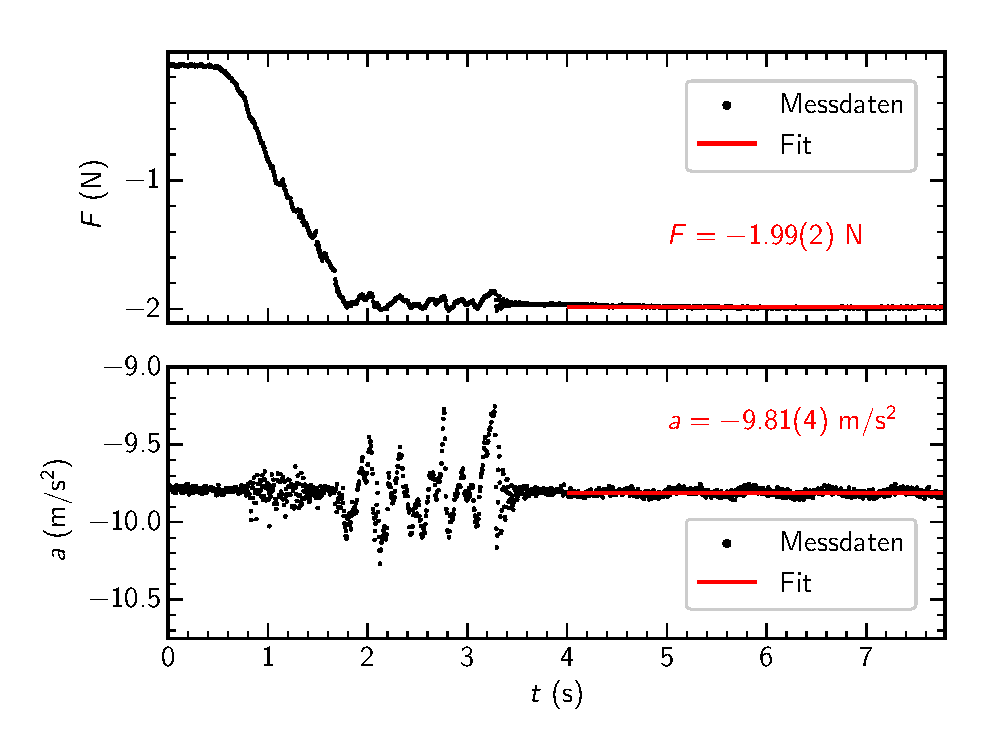
\includegraphics[width=\textwidth]{mass.eps}
	\caption[Bestimmung der Masse]{Vom oben nach unten sind Kraft \( F \) und Beschleunigung \( a \) aufgetragen. Die Fehlerbalken der Daten sind zu klein, um sie auszumachen und werden daher nicht eingetragen. Die zwei Grafiken teilen sich die horizontale Achse. Zudem sind in rot Geraden von \( t = 4 \unit{s} \) bis \( t = 8 \unit{s} \) angepasst.}
	\label{fig:mass}
\end{figure}

Der bestimmte Wert mit Fehler ist sowohl in der Abbildung, als auch in \autoref{table:1} zu sehen. Die Unsicherheit wurde auf die Standardabweichung der Daten gesetzt, da dann (per Definition) zwei Drittel der Daten innerhalb des \( 1\sigma \) Intervalls liegen.

\newpage
\begin{center}
	\captionaboveof{table}[Messdaten zur Massenbestimmung]{Gemessene Beschleunigung und Kraft und die daraus errechnete Masse der drei Versuche.}
	\begin{tabular}{@{\extracolsep{5mm}} 
			r
			S[table-format=1.2(1)]
			S[table-format=1.2(1)]
			S[table-format=1.2(1)]
		}
		\toprule
		\makecell[t]{}
		&   {\makecell[t]{Versuch 1}}
		&   {\makecell[t]{Versuch 2}}
		&   {\makecell[t]{Versuch 3}}\\
		\midrule
		\( a \unit{(\a)} \) & -9.81(4) & -9.73(6) & -9.81(8) \\
		\( F  \unit{(N)} \) & -1.99(2) & -2.78(2) & -3.93(7) \\
		\( m \unit{(kg)} \) & 0.202(2) & 0.286(3) & 0.400(7) \\
		\bottomrule
	\end{tabular}
	\label{table:1}
\end{center}

\section{Federpendel mit einer Feder}
\label{sec:Feder 1}
Für die Analyse der Oszillation wurde der Beschleunigungssensor verwendet, da dieser eine höhere Auflösung als der Kraftsensor besitzt. In \autoref{fig:sine} sind die Schwingungsdaten der zweiten Masse \( m_2 \) dargestellt. Links sind die ersten fünf Sekunden, in welchen „schöne” Schwingungen auftreten, zu sehen, während rechts die letzten Sekunden der Messung aufgetragen sind. In rot wurde eine Sinuskurve der Form \( f(x) = A\sin(\omega x + \phi) + d \) an die gesamten Messdaten von \( t = 4 \unit{s} \) bis \( t = 27 \unit{s} \) angepasst. 
	
\begin{figure}[H]
	\centering
	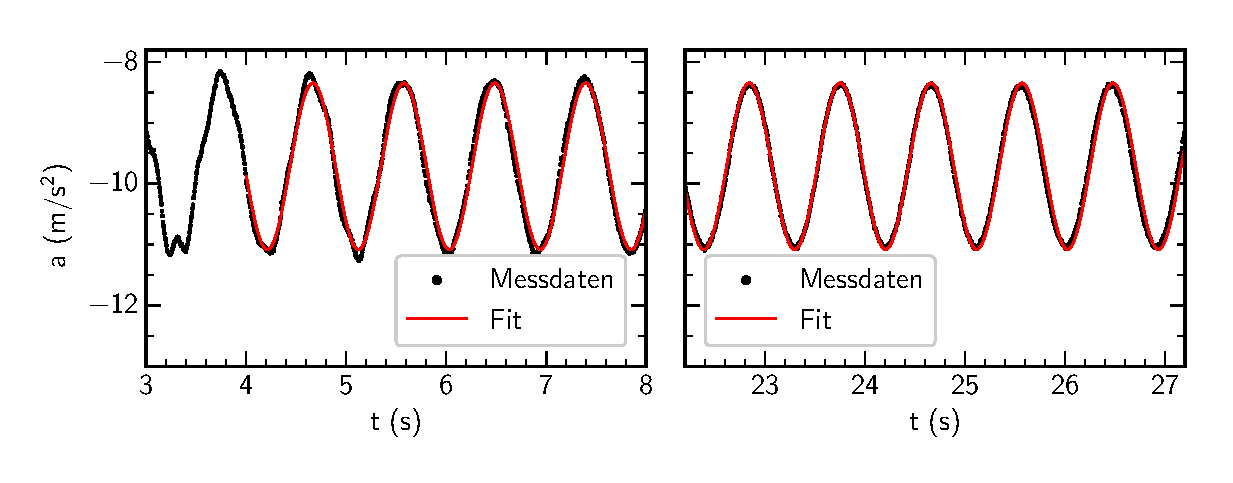
\includegraphics[width=\textwidth]{Feder1.eps}
	\caption[Oszillation mit einer Feder]{Die Beschleunigung wurde auf die Zeit aufgetragen und eine durchgehende Sinuskurve in rot wurde an die Daten ab \( t = 4 \unit{s} \) (bis \( t = 27 \unit{s} \)) angepasst. Dargestellt werden aber nur ersten 5 Sekunden (links) beziehungsweise letzten 5 Sekunden (rechts). Die Fehlerbalken der Daten sind zu klein, um sie auszumachen und werden daher nicht eingetragen.}
	\label{fig:sine}
\end{figure}
	
Aus dem Fit lässt sich direkt die Winkelfrequenz \( \omega \) mitsamt Fehler herauslesen. Aus dieser kann man wiederum mit \autoref{eqn:T} die Schwingungsdauer berechnen. In \autoref{table:2} sind charakteristische Eigenschaften der Schwingung, wie die Kreisfrequenz oder die Masse, eingetragen. 
	
\begin{center}
	\captionaboveof{table}[Messdaten zur Oszillation einer Feder]{Gemessene Masse, Schwingungsdauer, Winkelfrequenz und Federkonstante der drei Versuche.}
	\begin{tabular}{@{\extracolsep{5mm}} 
			r
			S[table-format=1.3(1)]
			S[table-format=1.3(1)]
			S[table-format=1.3(1)]
		}
		\toprule
		\makecell[t]{}
		&   {\makecell[t]{Versuch 1}}
		&   {\makecell[t]{Versuch 2}}
		&   {\makecell[t]{Versuch 3}}\\
		\midrule
		\( m \unit{(kg)}\) & 0.202(2) & 0.286(3) & 0.400(7) \\
		\( \tilde{m} \unit{(\sqrt{1/kg})} \) & 2.223(10) & 1.8698(99) & 1.580(15) \\
		\( T \unit{(s)} \) & 0.749(2) & 0.909(5) & 1.063(10) \\
		$\omega \unit{(1/s)}$ & 8.387(40) & 6.915(79) & 5.91(11) \\
		\( k \unit{(N/m)} \) & 14.2(2) & 13.7(3) & 14.0(6) \\
		\bottomrule
	\end{tabular}
	\label{table:2}
\end{center}

Das Modell des harmonischen Oszillators (Siehe \autoref{eqn:omega}) stellt einen linearen Zusammenhang zwischen \( \omega \) und der angepassten Masse \( \tilde{m} \) her mit\( \sqrt{k} \) als Proportionalitätskonstante. Dies wird in \autoref{fig:k1} anhand der in \autoref{table:1} angegebenen Werten illustriert. Zusätzlich zu den drei Datenpunkten wurde eine Gerade, wie sie das Modell vorhersagt, angepasst, wodurch man für die Steigung der linearen Funktion \( \sqrt{k} = 3.74(2) \unit{\sqrt{kg / s^2}} \) erhält. Nachdem wir kein Indiz dafür haben, dass die Gerade die Ordinate nicht im Ursprung schneidet, wurde der Fit gezielt mit nur einem Parameter (der Steigung) durchgeführt, um die Anzahl der Freiheitsgrade von 1 auf 2 zu erhöhen. 

\begin{figure}[H]
	\centering
	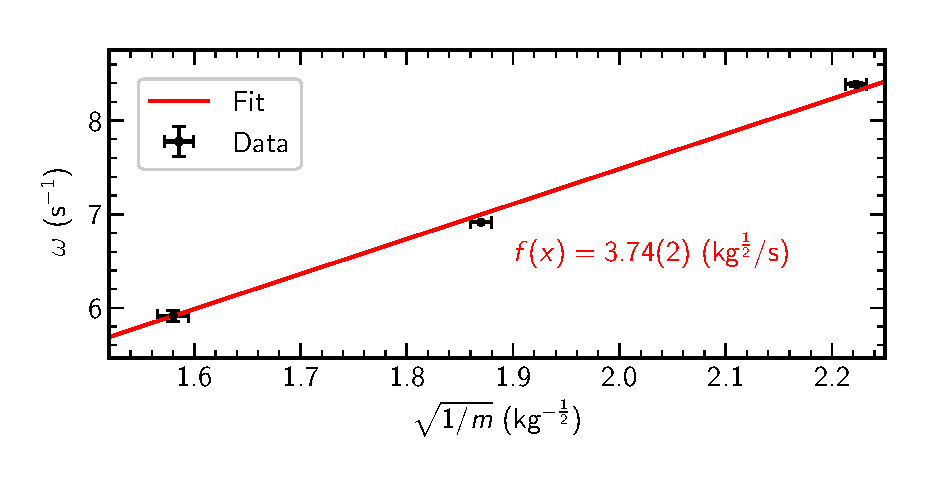
\includegraphics[width=\textwidth]{k1.eps}
	\caption[Zusammenhang zwischen \( \omega \) und \( \tilde{m} \)]{Die Winkelfrequenz der Schwingungen auf die angepasste Masse aufgetragen. In rot wurde eine lineare Funktion durch den Ursprung angepasst. Die Fehlerbalken stellen den $1\sigma$ Fehler dar.}
	\label{fig:k1}
\end{figure}

Für den Fit erhält man einen Chi-Quadrat Wert von \( \chi^2 = 4.22 \), woraus sich für das reduzierte Chi-Quadrat \( \chi_{\nu}^2 = 2.11 \) ergibt. Dieser Wert weicht zwar vom Erwartungswert ab, aber nicht signifikant. Es könnte aber darauf hindeuten, dass die Fehler zu klein abgeschätzt wurden, beziehungsweise Fehlerquellen nicht berücksichtigt wurden. 

Quadriert man nun den erhaltenen Fitparameter \( \sqrt{k} = 3.74(2) \unit{\sqrt{kg / s^2}} \) erhält man die Federkonstante \( k = 14.00(17) \unit{N/m} \). Wie in \autoref{sec:theorie} diskutiert ist die Federkonstante eine intrinsische Größe der Feder und hängt daher nicht von der angehängten Masse ab. Mittels \autoref{eqn:omega} kann man \( k \) für die drei Messungen mit unterschiedlichen Massen berechnen und man erwartet, dass sich die gleiche Konstante ergibt, was im Rahmen der Unsicherheit auch der Fall ist (Werte \autoref{table:2} entnehmen). 

In \autoref{fig:kFit} wurden in schwarz die Federkonstanten der drei Massen als normalisierte Gaußkurven aufgetragen. In rot ist die Federkonstante dargestellt, welche aus der Anpassung der linearen Funktion hervorgegangen ist.
\begin{figure}[H]
	\centering
	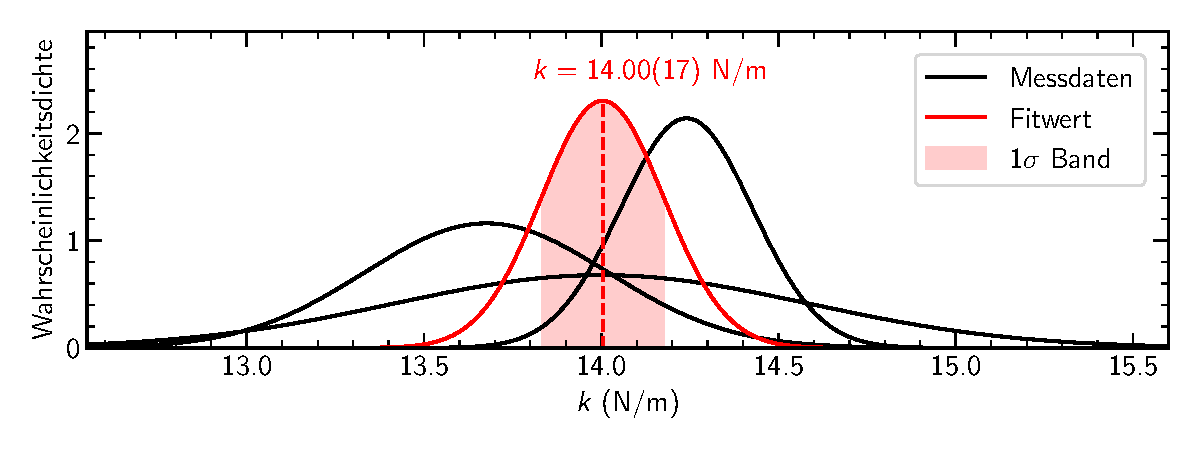
\includegraphics[width=\textwidth]{kFit.pdf}
	\caption[Vergleich der Federkonstanten als normalisierte Gaußkurven]{Die berechneten Federkonstanten der drei Massen wurden als normalisierte Gaußkurven in schwarz auf die Federkonstante aufgetragen. In Rot wurde das Quadrat der Steigung aus dem linearen Fit eingezeichnet. Das \( 1\sigma \) Intervall des Mittelwerts wurde farblich hinterlegt.}
	\label{fig:kFit}
\end{figure}

Der Fitparameter aus \autoref{fig:k1} in rot (kann man sich als Art Mittelwert der drei schwarzen Kurven vorstellen) passt gut zu den Daten, da alle Daten auf jeden Fall innerhalb des \( 2\sigma \) Intervalls liegen. Er schließt die Messungen nicht aus und bestätigt soweit die Annahme, dass es sich beim Federpendel um einen harmonischen Oszillator handelt. 


\section{Federpendel mit zwei Federn}

Im folgenden Versuch wurde die Masse \( m_3 = 0.400(7) \unit{kg} \) an zwei Federn gehängt. Die Schwingungsdaten wurden analog wie mit einer Feder analysiert, sprich es wurde eine Sinuskurve an die Beschleunigungsdaten angepasst, aus welcher sich die Kreisfrequenz \( \omega \) samt Fehler ablesen lässt. Mittels \autoref{eqn:omega} wurde anschließend die Gesamtfederkonstante des Systems ausgerechnet.
In \autoref{table:3} sind die Daten dargestellt.

\begin{center}
	\captionof{table}[Messdaten zur Oszillazion bei 2 Federn]{Gemessene Schwingungsdauer, Winkelfrequenz, Federkonstante und normierte Federkonstante bei einer und zwei Federn}
	\begin{tabular}{@{\extracolsep{5mm}} 
			r
			S[table-format=1.3(1)]
			S[table-format=1.2(1)]
			S[table-format=2.1(1)]
			S[table-format=2.1(1)]
		}
		\toprule
		\makecell[t]{}
		&   {\makecell[t]{\( T \unit{(s)} \)}}
		&   {\makecell[t]{\( \omega \unit{(1/s)} \)}}
		&   {\makecell[t]{\( k \unit{(N/m)}\)}}
		&   {\makecell[t]{\( k/N \unit{(N/m)}\)}}\\
		\midrule
		
		1 Feder & 1.063(10) & 5.91(11) & 14.0(6) & 14.0(6) \\
		2 Feder & 0.758(2) & 8.29(2) & 27.5(5) & 13.8(3) \\
%		3 Feder & 0.6193(10) & 10.15(2) & 41.2(8) & 13.7(3) \\
		\bottomrule
	\end{tabular}
	\label{table:3}
\end{center}

Wenn man die Federkonstanten der beiden Systeme vergleicht, fällt auf, dass die Konstante \( k_2 \) von zwei Federn im Rahmen der Unsicherheit doppelt so groß ist wie die einer Feder. Teilt man die Federkonstante durch die Anzahl der Federn \( k/N \) erhält man für beide Systeme den gleichen Wert (innerhalb der statistischen Abweichungen). Man könnte daher annehmen, dass das Superpositionsprinzip anwendbar ist und sich daher ergibt
\begin{equation}\label{eqn:paral1}
	k_{\text{ges}} = \sum_{i}^{N} k_i
\end{equation}
In diesem Versuch wird angenommen, dass alle Federn die gleichen Materialeigenschaften und daher die gleiche Federkonstante besitzen, wodurch sich \autoref{eqn:paral1} zu
\begin{equation}\label{eqn:paral2}
	k_{\text{ges}} = Nk
\end{equation}
vereinfacht, wobei \( k = 14.00(17) \unit{N/m} \) die in \autoref{sec:Feder 1} ermittelte Federkonstante ist. In einem System mit identen Federn skaliert also die Gesamtfederkonstante linear mit der Anzahl \( N \) der Federn.

\section{Testen des Modells}
Der letzte Versuch hat darauf abgezielt, das erstellte Modell mit einem System von drei Federn zu testen. Es wurde die gleiche Masse \( m_3 = 0.400(7) \unit{kg} \) wie mit zwei Federn verwendet und die Analyse der Schwingungen verlief analog. Es wurde eine Winkelfrequenz von \( \omega = 0.6193(10) \unit{1/s} \) ermittelt.

Bei \( N = 3 \) Federn sagt das Modell einen Wert von \( \hat{k}_3 = 42.0(1.8) \unit{N/m} \) vor, wobei empirisch ein Wert von \( k_3 = 41.2(8) \unit{N/m} \) ermittelt wurde. Sieht man sich die Differenz dieser beiden Größen an findet man, dass
\begin{equation}\label{eqn:diff}
	\hat{k}_3 - k_3 = 0.8(9) \unit{N/m}
\end{equation}
die Abweichung vom Modell nimmt im Rahmen der Unsicherheit den Wert 0 an und kann daher reiner statistischer Natur sein. Das Modell wird somit für Federn mit gleicher Federkonstante bestätigt.






